%!TEX program = pdflatex
\documentclass[UTF8]{article}

\usepackage[UTF8]{ctex}
\usepackage{enumerate}
\usepackage{graphicx}

\title{第五、六章作业}
\author{SA18225036 陈旻}
\begin{document}
\date{}
\maketitle
\section{第五章}
\subsection{第18题}
\paragraph{答案}
n=8+3=19,为求首地址,我们将,我们将 IP 地址 左边 19 位不变,右边全部置0,得 131.134.96.0。 求末地址 ,将 IP 地址左边19 位不变,右边全部置1,得131.134.127.255
\subsection{第26题}
\paragraph{答案}
不行,应总共发送2个帧,第一帧1500字节,第二帧46字节。
\subsection{第26题}
\paragraph{答案}
\begin{enumerate}[a.]
    \item 易得 $ n = 24 + log_{10}32 = 29  $,子网掩码即为 255.255.255.248
    \item 每个子网地址数为2的3次幂,即为8
    \item 第一个子网的首地址为 211.17.180.0/29 ,末地址为211.17.180.7/29 
    \item 最后一个子网的首地址为211.17.180.248/29,末地址为211.17.180.255/29
\end{enumerate}
\subsection{第33题}
\paragraph{答案}
~\\
第一组,200用户,每个需要128个地址,150.80.0.0/25——150.80.99.255/25 \\
第二组,400用户,每个需要16个地址,150.80.100.0/28——150.80.124.255/28 \\
第三组,2000用户,每个需要4个地址,150.80.125.0/30——150.80.156.255/30 \\
还剩下可用的地址数为$ 2^16-(200*128+400*16+2000*4)=25344 $
\section{第六章}
\subsection{第3题}
\paragraph{答案}
\begin{tabular}{|c|c|c|}
    \hline \multicolumn{3}{|c|}{A类}\\
    \hline 网络地址&下一跳地址&接口\\
    \hline 111.0.0.0&---&m1\\
    \hline \multicolumn{3}{|c|}{B类}\\
    \hline 网络地址&下一跳地址&接口\\
    \hline 145.80.0.0&111.25.19.201&m1\\
    \hline 170.14.0.0&111.25.19.201&m1\\
    \hline \multicolumn{3}{|c|}{C类}\\
    \hline 网络地址&下一跳地址&接口\\
    \hline 192.16.7.0 &111.15.17.32&m1\\
    \hline \multicolumn{3}{|c|}{}\\
    \hline 默认的 &无下一跳&m0\\
    \hline
\end{tabular}
\subsection{第10题}
\paragraph{答案}
~\\
最长前缀匹配到201.4.16.0/22,即R1路由通过接口m1进行转发。
\subsection{第14题}
\paragraph{答案}
见文末图
\begin{figure}[h]
    \begin{center}
        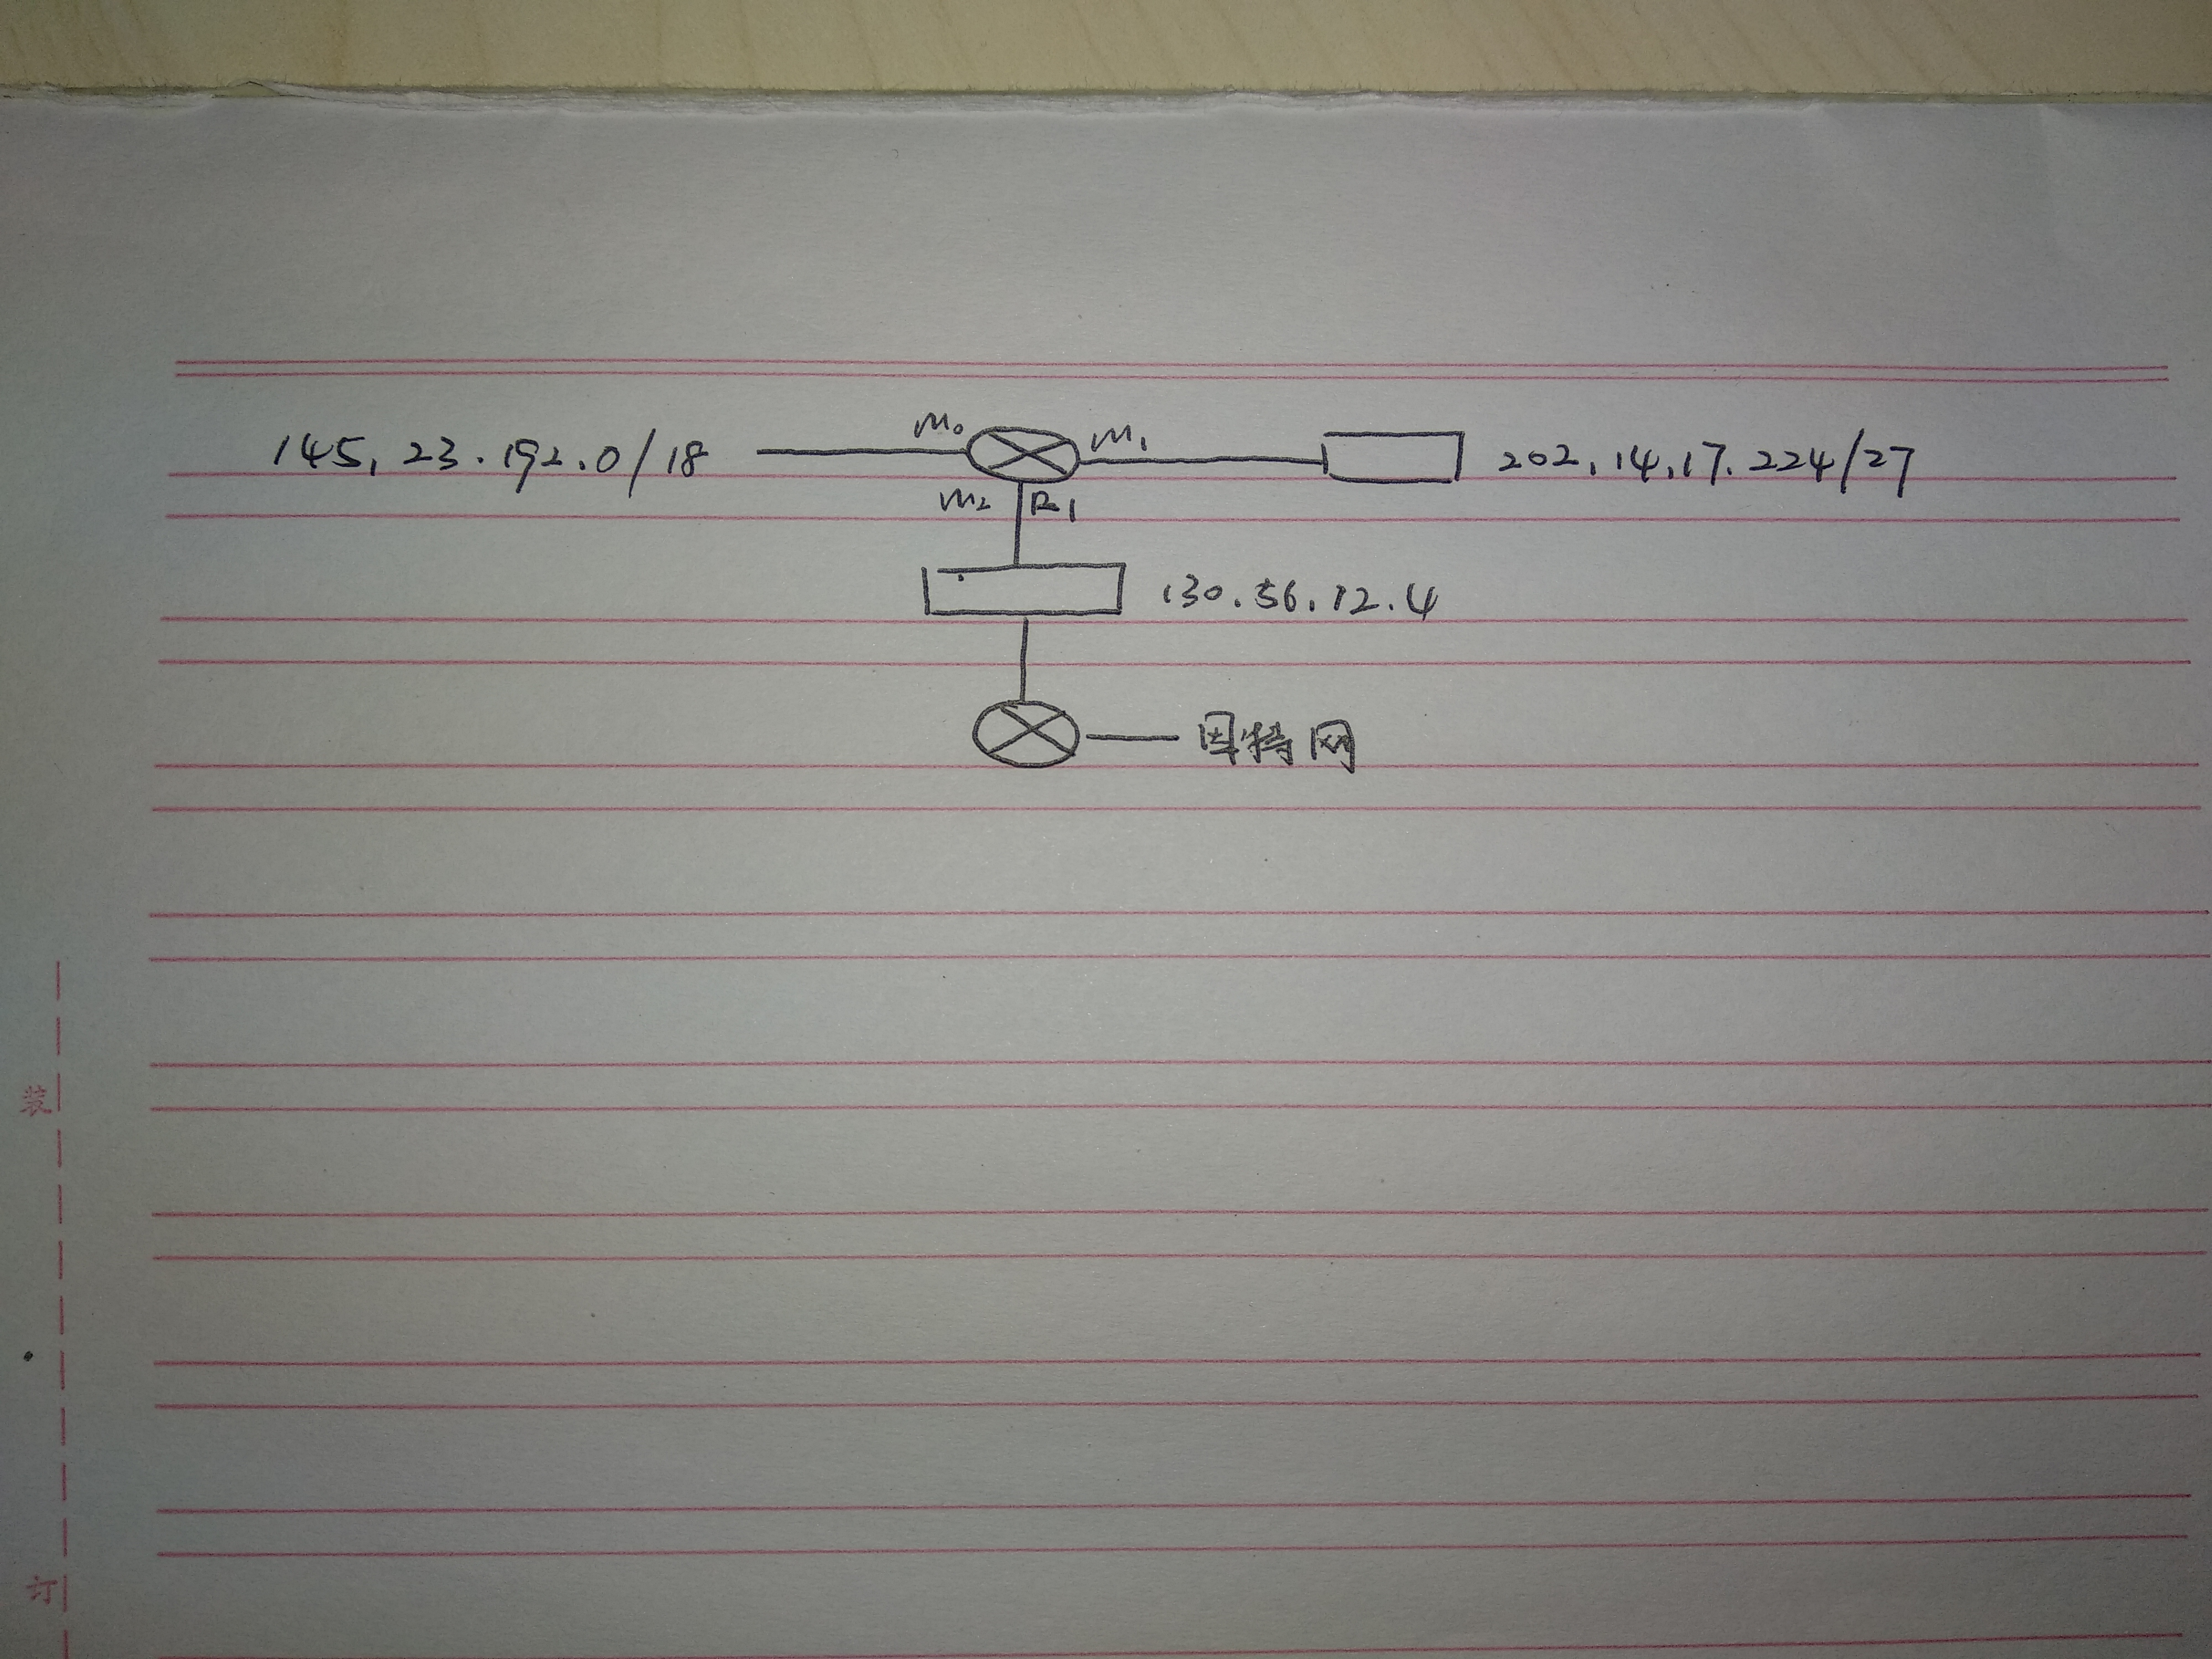
\includegraphics[scale=0.1]{img/ch6_14.jpg}
    \end{center}
\end{figure}
\subsection{第15题}
\paragraph{答案}
~\\
能。当分组从组织1、2、3传来的时候,R1先收到,再从 m3 接口转发走。如果分组先传给R2,会从m1接口传给R3,R3再从m0接口传走,R1收不到。如果分组先传给R3,R3直接从m0接口传走,R1也收不到。
\end{document}